% This is samplepaper.tex, a sample chapter demonstrating the
% LLNCS macro package for Springer Computer Science proceedings;
% Version 2.20 of 2017/10/04
%
\documentclass[runningheads]{llncs}
%
\usepackage{graphicx}
\usepackage{listings}
\usepackage{wrapfig}
% Used for displaying a sample figure. If possible, figure files should
% be included in EPS format.
%
% If you use the hyperref package, please uncomment the following line
% to display URLs in blue roman font according to Springer's eBook style:
% \renewcommand\UrlFont{\color{blue}\rmfamily}

\begin{document}
%
\title{Marlowe: implementing and analysing financial contracts\thanks{Supported by IOHK.}}
%
%\titlerunning{Abbreviated paper title}
% If the paper title is too long for the running head, you can set
% an abbreviated paper title here
%
\author{
Pablo {Lamela Seijas}\inst{1} \and
Alex Nemish\inst{1} \and
David Smith\inst{1} \and
Simon Thompson\inst{1,2}\orcidID{0000-0002-2350-301X}}
%
\authorrunning{P. Lamela Seijas, A. Nemish, et al.}

% First names are abbreviated in the running head.
% If there are more than two authors, 'et al.' is used.
%
\institute{IOHK, Hong Kong, \url{https://iohk.io} \\
\email{\{alexander.nemish, pablo.lamela, david.smith, simon.thompson\}@iohk.io} \and
School of Computing, University of Kent, UK\\
\email{s.j.thompson@kent.ac.uk}}
%
\maketitle              % typeset the header of the contribution
%



\begin{abstract}
The abstract should briefly summarize the contents of the paper in
150--250 words.

\keywords{First keyword  \and Second keyword \and Another keyword.}
\end{abstract}
%
%
%


\section{Introduction}

Intro
\section{Marlowe overview SJT}

Introduce the main types and informal overview of execution. Contrast with Marlowe 1.3 (as in ISoLA paper). Embedding in Haskell? [All this stuff is in the tutorial already]

\section{Implementation of Marlowe on the mockchain AN}

 [An updated version of the description in the Plutus platform paper]

\section{Analysing Marlowe\label{sec:analysis}}

In this section, we give an overview of some of the work we have carried out with the aim of helping users be more confident in that the Marlowe contracts they write do what they expect them to do.

We look at two complementary approaches: static analysis of concrete contracts (Section~\ref{subsec:static}) and formal verification of general properties about Marlowe (Section~\ref{subsec:verification}).

\subsection{Static analysis of contracts\label{subsec:static}}

For some properties, and given a particular contract, a computer can decidably determine whether the contract satisfies the property and, in the cases when it does not, it can provide a counter example.

For turing-complete languages, this process is often undecidable in the general case. And for Marlowe contracts it is often NP-complete in the general case. However, in practice, SAT solvers are often able to solve moderately large instances of this problem reasonably efficiently.

Our implementation relies on the Haskell library SBV, which in turn relies on existing SAT solvers for proving satisfiability of properties or finding counter examples.

\subsubsection{SBV library}

SBV (SMT Base Verificiation) library provides a high-level API that allows developers to automatically prove properties about Haskell programs, among other functionalities.

The SBV library seamlessly translates these property to SMTLib queries, passes them to one or several SAT solvers, and translates the results back to the format in which the queries were written.

\paragraph{\texttt{SBV} monad.}

SBV provides a monad called \texttt{SBV} which encapsulates potentially unknown values to the program. A program that takes arguments wrapped with the \texttt{SBV} monad can be used with normal arguments and it can also be passed symbolic parameters when used as part of a property that is passed to the solver.

For example, the following function:

\begin{verbatim}
primeFactors :: SBV Integer -> SBV Integer -> SBV Bool
primeFactors x y = x .> 1 .&& y .> 1 .=> x * y ./= 25723297
\end{verbatim}

can be used both with normal integers and with symbolic parameters:

\begin{verbatim}
*Main> primeFactors 98 314
True
*Main> prove primeFactors
Falsifiable. Counter-example:
    s0 = 6353 :: Integer
    s1 = 4049 :: Integer
*Main> primeFactors 6353 4049
False
\end{verbatim}

\paragraph{Limitations}

At the time of writing, there are some types of functions and data-types that SBV cannot translate to \texttt{SMTLib}. In particular, there are two that affected the way in which we use SBV with Marlowe and that prevent us from using the same version of the semantics for symbolic execution and normal execution.

Firstly, recursive functions that are unbound cannot be translated. As part of the process of converting functions to \texttt{SMTLib} terms, SBV unfolds them into a finite data-structure. For this reason, if the function is recursive and is not bounded by a non-symbolic value (a value that is known at the time of translation), the translation process will run out of memory.

Secondly, to the best our knowledge, SBV does not currently provide support for custom data types directly (except for non-ary datatypes, i.e: enumerations).

In the following section, we explain how we worked around these limitations and overview how we use SBV to avoid runtime problems with Marlowe contracts.

\subsubsection{Using SBV to analyse Marlowe Contracts}

Marlowe semantics are designed to use types to prevent many non-sensical contracts from being written. But there are potential problems which are harder to notice until runtime (e.g: whether there will be enough money to issue all the payments declared in the contract), at which point it may already be too late to fix them (in the case of blockchain). Marlowe semantics represents these errors that can be found at runtime as \texttt{Warnings}.

The property that we have implemented using SBV library can be enunciated as: "the given contract will not need to issue warnings in runtime no matter the inputs it receives".

In order to achieve this, we implemented a symbolic version of the semantics that returns a list of the warnings produced by a trace (a list of transactions input to the contract):

\begin{verbatim}
warningsTraceWB :: Bounds -> SSlotNumber -> SList NTransaction
                -> Contract -> SList NTransactionWarning
\end{verbatim}

Where types that start with \texttt{S} like \texttt{SSlotNumber} are abreviations for the symbolic versions of types (in this case \texttt{SBV SlotNumber}).

The types that start with \texttt{N} are \textit{nested} types, which we explain later in the \textit{Custom datatypes} section below.

We can see that this version of the implementation takes two concrete parameters: \texttt{Bounds} (with info about the bounds of the contract) and \texttt{Contract} (the contract we want to analyse); and two symbolic parameters: \texttt{SSlotNumber} (the initial slot number) and \texttt{SList NTransaction} (the input list of transactions); and it returns \texttt{SList NTransactionWarning} (a symbolic list of transaction warnings).

\paragraph{Custom datatypes}

As we mentioned before, SBV does not currently seem to support in general the use of custom datatypes. We do not need to represent the \texttt{Contract} type symbolically because we know its value at the time of analysis, but we still have many other types like \texttt{TransactionWarning} that are custom datatypes and we need to use.

Fortunately, SBV does support tuples and the \texttt{Either} type; combinations of those two give us essentially the same functionality as custom datatypes that are not recursive and have no type-parameters. We can represent all types that Marlowe requires as combinations of \texttt{Either} and tuples, with the exception of the \texttt{Contract} type, but we do not need a symbolic version of the \texttt{Contract} type.

For example, the TransactionResult type:
\begin{verbatim}
data TransactionResult = TransactionProcessed [TransactionWarning]
                                              [TransactionEffect]
                                              State
                       | TransactionError TransactionError
\end{verbatim}

becomes the nested type synonym \texttt{NTransactionResult}:

\begin{verbatim}
type NTransactionResult =
      Either ([NTransactionWarning], [NTransactionEffect], NState)
             NTransactionError
\end{verbatim}

Because working with nested types is much more error prone than working with the original data-types, we used template haskell to implement functions that transform the custom datatypes into nested types and generates the appropriate conversion functions.

\paragraph{Returning non-symbolic \texttt{Contract} values}

In the original semantics, each step typically takes a \texttt{Contract}, a \texttt{State}, and a set of \texttt{Input}s; and it returns an updated \texttt{State} and a remaining \texttt{Contract}. This is a problem because values that rely on symbolic values, have to be themselves symbolic. And the resulting remaining \texttt{Contract} depends on the \texttt{Input}s and \texttt{State} which are both symbolic.

We work around this problem by slightly modifying the signature of the function to receive a \textit{continuation function} instead; and instead of just returning a value, we return the result of applying the \textit{continuation function} to the result we were planning to return.

For example, the original type signature for the \texttt{apply} function was:

\begin{verbatim}
apply :: Environment -> State -> Input -> Contract -> ApplyResult
\end{verbatim}

But the symbolic version of the \texttt{apply} function has the following signature:

\begin{verbatim}
apply :: SymVal a => Bounds -> SEnvironment -> SState -> SInput
      -> Contract -> (SApplyResult -> DetApplyResult -> SBV a)
      -> SBV a
\end{verbatim}

Where \texttt{DetApplyResult} contains the parts of \texttt{ApplyResult} that are not symbolic (like the \texttt{Contract}).

\paragraph{Bounds for the state and the inputs}

The recursion in the execution of the semantics is bounded by the \texttt{Contract}, and because the \texttt{Contract} is not a symbolic parameter, the translation will terminate.

However, both in the input and in the \texttt{State} record there are several lists (or association maps) that are not explicitly bounded in the implementation. Some parts of the semantics are bounded by the length of these lists (or maps), like the implementation of \texttt{Close} that refund all the money available in all the accounts.

In order for the symbolic implementation to be finite we need to find a bound for the length of these lists and maps.

With the current semantics of Marlowe all of the lists/maps in State and input can be bound when looking at a particular contract. In particular, we can find out quite easily, by looking at the contract, how many parties there are, how many choice identifiers are used, how many accounts are used, and how many let binding identifiers are used.

It is less obvious that we can also set a bound for the input \texttt{Transaction} list as the maximum number of nested \texttt{When}s in the contract (for all the execution paths) plus one. We also provide a proof in Isabelle that shows that any longer list of transactions will result in an error, Since transactions that result on errors do not modify the \texttt{State} or the \texttt{Contract}, we know that limiting the analysis to lists of transactions that are shorter than the bound does not lose generality.

\subsection{Formal verification of semantics\label{subsec:verification}}

We can also use proof assistants like Isabelle to demonstrate that Marlowe semantics present certain desirable properties (like that money is preserved and returned to users by the end of the execution of any contract). In the same way, we can also use this technique to prove properties for particular contracts, or for particular contract snippets, templates, or classes of contracts.

\clearpage
\section{The Marlowe Playground}

For Marlowe to be usable in practice, users need to be able to understand how contracts will behave once deployed to the blockchain before actually deploying the contract. We can do that by simulating their behavior with a mockchain and interactively stepping through the evaluation of a contract in a browser.

To achieve this, and to aid Marlowe’s take-up usage by people who are not familiar with its syntax, we have developed the Marlowe Playground, a web tool that supports the interactive construction, revision, and simulation of smart-contracts written in Marlowe. The tool is publicly available in the url: https://prod.meadow.marlowe.iohkdev.io/. It should be mentioned that development of the playground is rapid and the latest unstable version is also publicly available at https://alpha.marlowe.iohkdev.io/.

The playground has an editor where you can write a contract in "pure" Marlowe, that is, not embedded in a host language. The reason for doing this is two-fold:
\begin{itemize}
    \item There is a shallower learning curve for users who are new to Haskell or programming languages in general. The Marlowe constructs are quite simple so there is no need to learn about Haskell syntax or even variables, functions etc.
    \item As we step through the execution of a contract, the contract is reduced, it is very useful to be able to view and even edit the reduced contract during this execution.
\end{itemize}
This is probably not the best way to write a large contract so the playground contains an additional editor where contracts can be written using Haskell and then transferred as a pure Marlowe data structure into the Marlowe editor.

In addition to pure Marlowe and Haskell editors, contracts can also be written using Google's Blockly visual programming language. Again this is not suitable for writing large contracts however it is an easy way to introduce the concepts of Marlowe to users who have no programming knowledge. Once a contract has been 'written' in Blockly it is possible to transfer that contract to the Marlowe editor. It is also possible to transfer a Marlowe contract to Blockly for further editing.

The Marlowe editor in the unstable version of the playground has an additional feature to aid writing contracts called holes. If we enter the contract \lstinline{?mycontract} we will be presented with a dropdown list of values that could be used.

\begin{wrapfigure}[5]{l}{0.25\textwidth}
    \vspace*{-0.3in}
    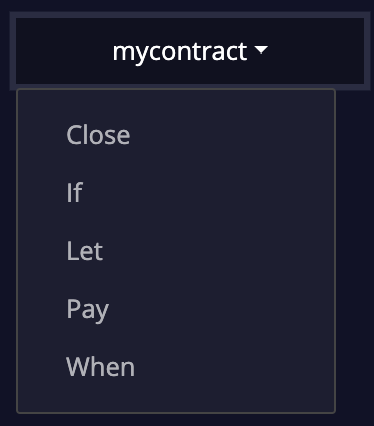
\includegraphics[width=0.25\textwidth]{hole_options.png}
\end{wrapfigure}
In our case \lstinline{?mycontract} must be a \lstinline{Contract} of some sort so we can choose one of the \lstinline{Contract} constructors from the dropdown list. If we choose \lstinline{Pay} then the Marlowe editor will automatically fill in a skeleton \lstinline{Pay} contract with new holes where we need to provide values.
\\ \\
\begin{verbatim}
    Pay ?accountId_1_1 ?payee_1_2 ?value_1_3 ?contract_1_4
\end{verbatim}
New options will be presented, one for each hole, and each will have a dropdown list of all the possible values.
\begin{wrapfigure}[6]{l}{0.25\textwidth}
    \vspace*{-0.3in}
    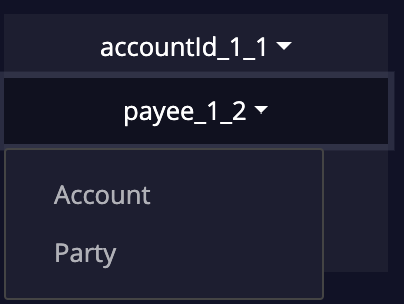
\includegraphics[scale=0.2]{hole_options_2.png}
\end{wrapfigure}
A complete contract can be written in this guided way with the user needing only to fill in strings and numbers by hand. This approach to writing holes in your code and "asking" the compiler what you could put in there is easy to implement in a DSL as there are very limited options however is is becoming popular with more complex languages such as Haskell and Idris.

Contracts written in the Marlowe editor are parsed in real-time and if there are no errors (and no holes) then the contract is analyzed to discover which actions a user could take to progress the contract. These actions are displayed in the "Input Composer" above the editor. Lets take the following example contract:
\begin{verbatim}
    When [Case (Deposit (AccountId 0 "investor") "guarantor" (Constant 1000)) 
    Close] 10 Close
\end{verbatim}
In this case, the only action a user can take to progress the contract is to deposit 1000 ADA from the guarantor to the investor's account. The playground knows this and so the input composer displays this action in the input composer.

\begin{figure}[]
    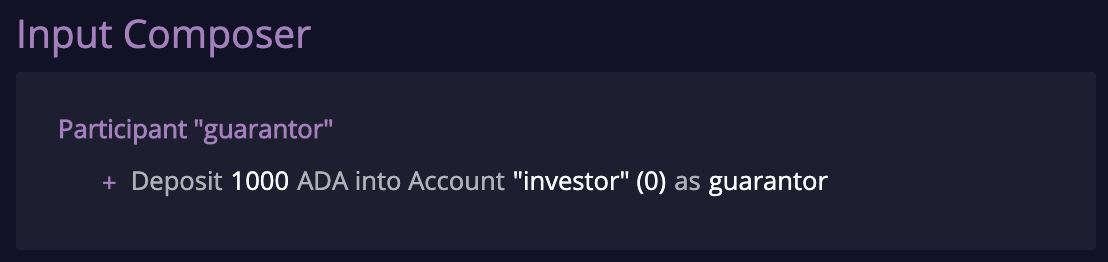
\includegraphics[width=1\textwidth]{input_composer.png}
\end{figure}
The user can then choose to add this action to a transaction, ready to be applied. Multiple actions can be added to a transaction before it is applied if such actions are meaningful.

\begin{figure}[]
    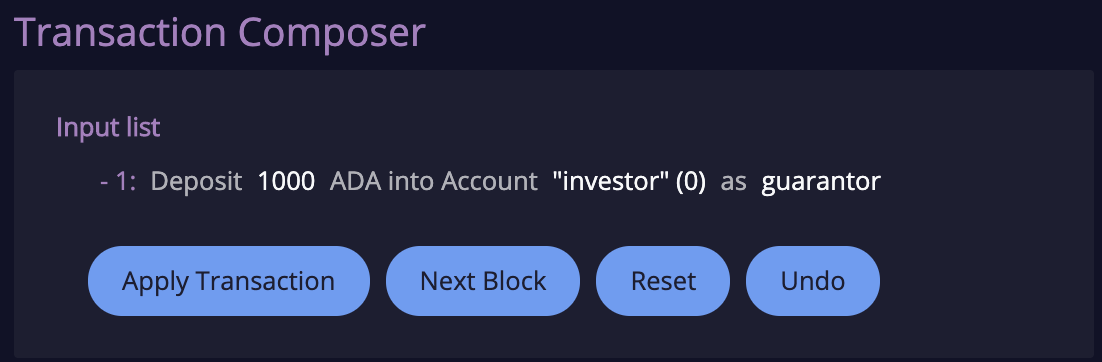
\includegraphics[width=0.8\textwidth]{tx_composer.png}
\end{figure}
A user can then apply this transaction and in the example above this would result in the state pane showing a single payment and in addition the Contract in the Marlowe editor will have been reduced to \lstinline{Close}. At this point a user can undo the application of the transaction or even reset the contract to it's initial state. This enables a user to apply transactions, see what the effect is, step back and apply a transaction with different actions and see how these differences effect the end results. They can also change the reduced contract to investigate a different path.

Users can at any point save their contract directly to a Github Gist and of course load a contract from a Github Gist. There are also some demo contracts that can be loaded in order to play around with realistic examples.

The final feature that we would like to present is the static analysis of contracts. As mentioned in a previous section, it is possible to carry out a symbolic execution of a contract and then use a SMT solver to look for cases that could cause unwanted situations. The playground utilizes this to search for situations where contract execution would cause warnings. For example, suppose you write a contract that causes a payment of 450 Lovelace from Alice to Bob but the contract allows a situation where Alice has only deposited 350 Lovelace then the static analysis will find this and report it to the playground user.
\begin{figure}
    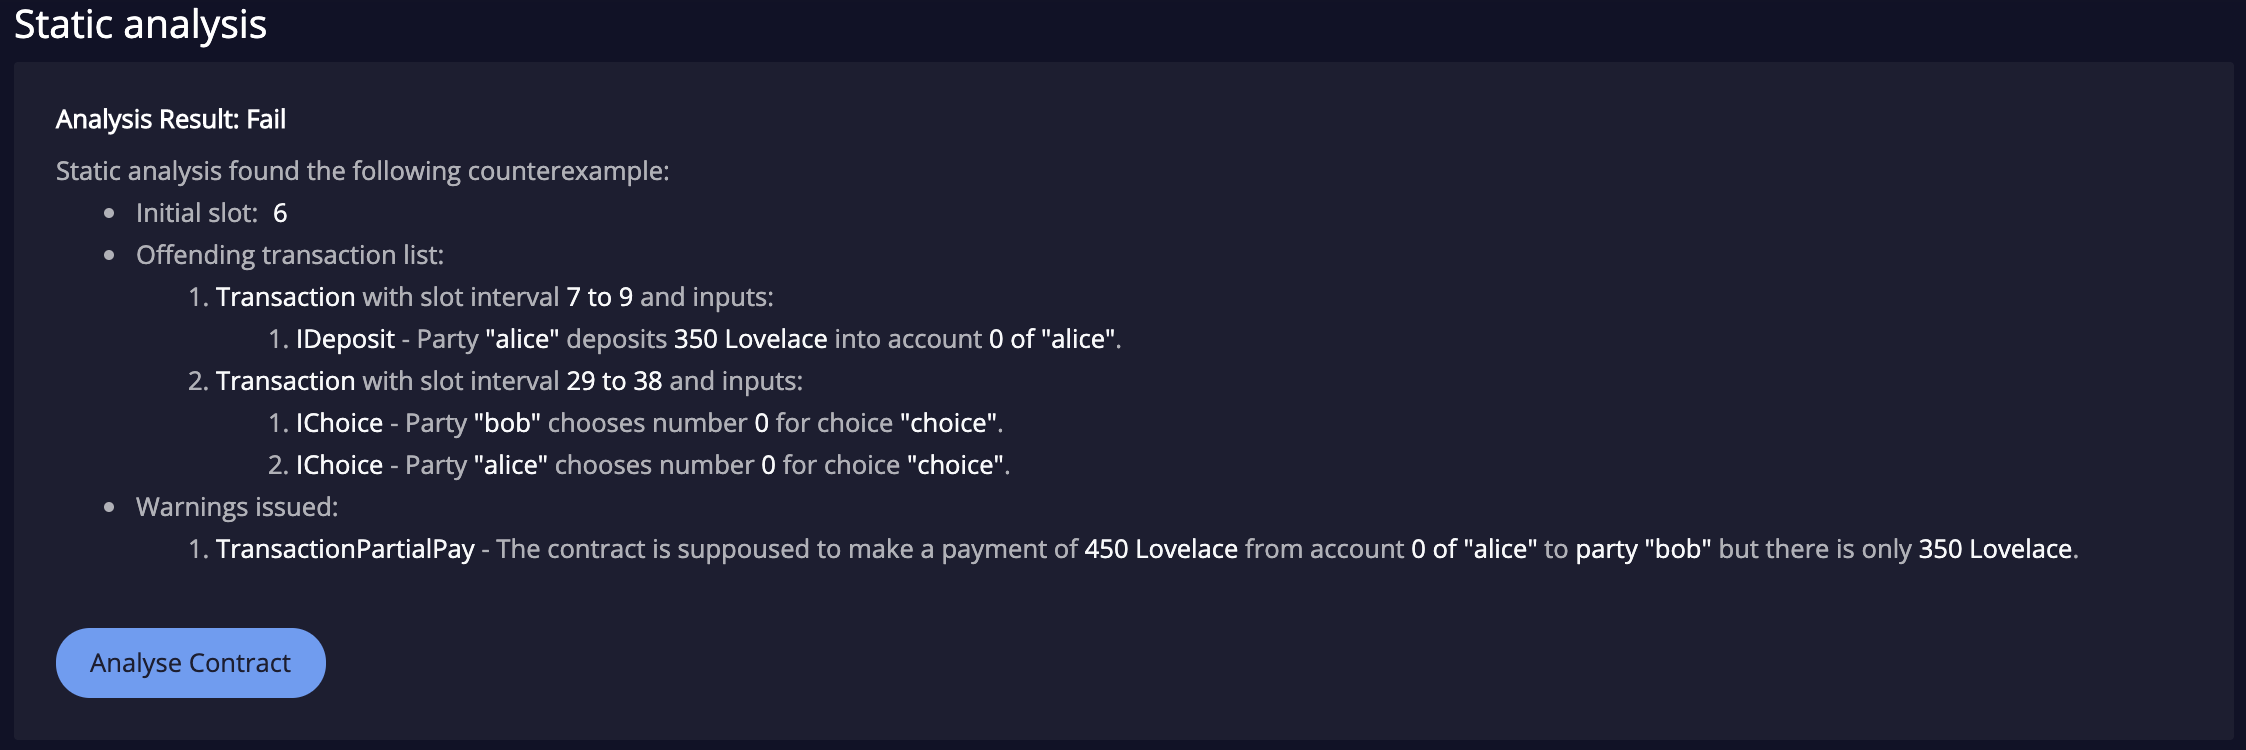
\includegraphics[width=1\textwidth]{static_analysis.png}
\end{figure}
\clearpage
\section{Related work}

Need to update from ISoLA paper \cite{isola-marlowe}.

\section{Future work and conclusions}

\section*{Left in for info \ldots}

\begin{figure}
% 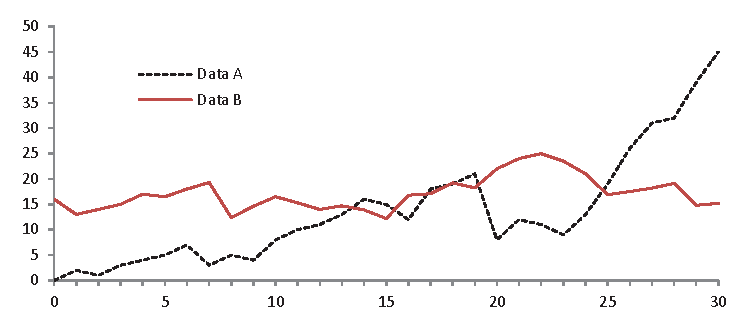
\includegraphics[width=\textwidth]{fig1.eps}
\caption{A figure caption is always placed below the illustration.
Please note that short captions are centered, while long ones are
justified by the macro package automatically.} \label{fig1}
\end{figure}


%
% ---- Bibliography ----
%
% BibTeX users should specify bibliography style 'splncs04'.
% References will then be sorted and formatted in the correct style.
%
\bibliographystyle{splncs04}
\bibliography{paper}
%
\end{document}
